% answers.tex —— 1990 年·全国卷·文科 · 参考答案与详细解析片段
% 由 tools/generate_projects.py 依来源总账自 1990/1990_数学真题_全国文_试题.md + 1990/1990_数学真题_全国文_解析正文.md + 1990/1990_数学真题_全国文_答案要点.md 生成，勿手改（改源 MD 后重跑）


\begin{gktip}
以下推导基于本项目题面转录，均为自行生成的解析，不是来源印载内容；26题独立盲核已完成。第 4 题初稿的复数乘法多写负号，已按复核更正为选项 B。第 20 题的几何计算仅确定两侧的无序体积比，因固定源没有标注 $V_1,V_2$ 对应区域，保留待核。
\end{gktip}

\begin{answer}
\gksolhead{1}{}

\textbf{题目}：

方程 $2^{\log_3 x}=\dfrac14$ 的解是\mbox{（　　）}。

（A）$x=\dfrac19$　　（B）$x=\dfrac{\sqrt3}{3}$　　（C）$x=\sqrt3$　　（D）$x=9$

\Needspace{4\baselineskip}
\textbf{解析}

令 $t=\log_3x$。由 $2^t=\frac14=2^{-2}$ 得 $t=-2$，所以 $x=3^{-2}=\frac19$。

\textbf{结论：A}

\gkanswer{答案：A}

\end{answer}
\begin{answer}
\gksolhead{2}{}

\textbf{题目}：

$\cos^2 75^\circ+\cos^2 15^\circ+\cos75^\circ\cos15^\circ$ 的值等于\mbox{（　　）}。

（A）$\dfrac{\sqrt6}{2}$　　（B）$\dfrac32$　　（C）$\dfrac54$　　（D）$1+\dfrac{\sqrt3}{4}$

\Needspace{4\baselineskip}
\textbf{解析}

\Needspace{5\baselineskip}
因为 $\cos75^\circ=\sin15^\circ$，前两项之和为 $\sin^215^\circ+\cos^215^\circ=1$；并且
\nopagebreak[4]
\[
\cos75^\circ\cos15^\circ=\sin15^\circ\cos15^\circ=\frac12\sin30^\circ=\frac14.
\]
原式为 $1+\frac14=\frac54$。

\textbf{结论：C}

\gkanswer{答案：C}

\end{answer}
\begin{answer}
\gksolhead{3}{}

\textbf{题目}：

如果轴截面为正方形的圆柱的侧面积是 $S$，那么圆柱的体积等于\mbox{（　　）}。

（A）$\dfrac S2\sqrt S$　　（B）$\dfrac S2\sqrt{\dfrac S\pi}$　　（C）$\dfrac S4\sqrt S$　　（D）$\dfrac S4\sqrt{\dfrac S\pi}$

\Needspace{4\baselineskip}
\textbf{解析}

\Needspace{5\baselineskip}
设圆柱半径为 $r$、高为 $h$。轴截面是正方形，故 $h=2r$。侧面积
\nopagebreak[4]
\[
S=2\pi rh=4\pi r^2,
\]
\Needspace{5\baselineskip}
体积为 $V=\pi r^2h=2\pi r^3$。由 $r=\sqrt{S/(4\pi)}$ 得
\nopagebreak[4]
\[
V=\frac S4\sqrt{\frac S\pi},
\]
对应选项D。

\textbf{结论：D}

\gkanswer{答案：D}

\end{answer}
\begin{answer}
\gksolhead{4}{}

\textbf{题目}：

把复数 $1+i$ 对应的向量按顺时针方向旋转 $\dfrac{2\pi}{3}$，所得向量对应的复数是\mbox{（　　）}。

（A）$\dfrac{1-\sqrt3}{2}+\dfrac{-1+\sqrt3}{2}i$　　（B）$\dfrac{-1+\sqrt3}{2}+\dfrac{-1-\sqrt3}{2}i$

（C）$\dfrac{-1+\sqrt3}{2}+\dfrac{1-\sqrt3}{2}i$　　（D）$\dfrac{1-\sqrt3}{2}+\dfrac{-1-\sqrt3}{2}i$

\Needspace{4\baselineskip}
\textbf{解析}

\Needspace{5\baselineskip}
顺时针旋转 $\frac{2\pi}{3}$ 等价于复数乘 $e^{-2\pi i/3}=-\frac12-\frac{\sqrt3}{2}i$，所以
\nopagebreak[4]
\[
(1+i)e^{-2\pi i/3}=\frac{-1+\sqrt3}{2}-\frac{1+\sqrt3}{2}i.
\]

\textbf{结论：B}

\gkanswer{答案：B}

\end{answer}
\begin{answer}
\gksolhead{5}{}

\textbf{题目}：

曲线 $\dfrac{y^2}{16}-\dfrac{x^2}{9}=1$ 的准线方程是\mbox{（　　）}。

（A）$y=\pm\dfrac{16}{\sqrt7}$　　（B）$x=\pm\dfrac{16}{\sqrt7}$　　（C）$y=\pm\dfrac{16}{5}$　　（D）$x=\pm\dfrac{16}{5}$

\Needspace{4\baselineskip}
\textbf{解析}

双曲线的半实轴 $a=4$、半虚轴 $b=3$，故 $c=\sqrt{a^2+b^2}=5$、离心率 $e=c/a=5/4$。纵轴双曲线的准线为 $y=\pm a/e$，即 $y=\pm16/5$。

\textbf{结论：C}

\gkanswer{答案：C}

\end{answer}
\begin{answer}
\gksolhead{6}{}

\textbf{题目}：

如图是函数 $y=2\sin(\omega x+\varphi)$（$|\varphi|<\dfrac\pi2$）的图象，那么\mbox{（　　）}。
\nopagebreak[4]
\begin{center}% 原卷第6题的正弦曲线及标注；依图重绘，曲线按函数形式绘出，非截图。
\begin{tikzpicture}[x=1.35cm,y=0.72cm,line cap=round,line join=round]
  \draw[->] (-0.38,0) -- (3.45,0) node[right] {$x$};
  \draw[->] (0,-2.25) -- (0,2.25) node[above] {$y$};
  \draw[thick,domain=-0.34:3.32,samples=140,smooth,variable=\t]
    plot (\t,{2*sin(2*\t r+30)});
  \draw (-0.06,1) -- (0.06,1);
  \node[left] at (-0.06,1) {$1$};
  \node[below left] at (0,0) {$O$};
  \node[below] at (2.879793,0) {$\dfrac{11\pi}{12}$};
\end{tikzpicture}
\end{center}
\nopagebreak[4]
（A）$\omega=\dfrac{10}{11},\ \varphi=\dfrac\pi6$　　（B）$\omega=\dfrac{10}{11},\ \varphi=-\dfrac\pi6$

（C）$\omega=2,\ \varphi=\dfrac\pi6$　　（D）$\omega=2,\ \varphi=-\dfrac\pi6$

\Needspace{4\baselineskip}
\textbf{解析}

\Needspace{5\baselineskip}
图象在 $x=0$ 处过点 $(0,1)$ 且递增。于是 $2\sin\varphi=1$，结合 $|\varphi|<\frac\pi2$ 得 $\varphi=\frac\pi6$。正弦曲线从 $x=0$ 起的第二个正零点满足 $\omega x+\varphi=2\pi$；题图标为 $x=\frac{11\pi}{12}$，故
\nopagebreak[4]
\[
\omega=\frac{2\pi-\pi/6}{11\pi/12}=2.
\]

\textbf{结论：C}

\gkanswer{答案：C}

\end{answer}
\begin{answer}
\gksolhead{7}{}

\textbf{题目}：

设命题甲为：$0<x<5$；命题乙为：$|x-2|<3$。那么\mbox{（　　）}。

（A）充分不必要条件　　（B）必要不充分条件　　（C）充要条件　　（D）既不充分也不必要条件

\Needspace{4\baselineskip}
\textbf{解析}

$|x-2|<3$ 等价于 $-1<x<5$。若 $0<x<5$，则必有 $-1<x<5$，所以甲能推出乙；反向不成立，例如 $x=-\frac12$ 满足乙但不满足甲。

\textbf{结论：A}

\gkanswer{答案：A}

\end{answer}
\begin{answer}
\gksolhead{8}{}

\textbf{题目}：

\Needspace{5\baselineskip}
函数
\nopagebreak[4]
\[
y=\frac{\sin x}{|\sin x|}+\frac{|\cos x|}{\cos x}+\frac{\tan x}{|\tan x|}+\frac{|\cot x|}{\cot x}
\]
的值域是\mbox{（　　）}。

（A）$\{-2,4\}$　　（B）$\{-2,0,4\}$　　（C）$\{-2,0,2,4\}$　　（D）$\{-4,-2,0,4\}$

\Needspace{4\baselineskip}
\textbf{解析}

在表达式有定义时令 $s=\operatorname{sgn}(\sin x)$、$c=\operatorname{sgn}(\cos x)$。则 $\operatorname{sgn}(\tan x)=\operatorname{sgn}(\cot x)=sc$，原式为 $s+c+2sc$。当 $(s,c)$ 取 $(1,1),(1,-1),(-1,1),(-1,-1)$ 时，所得值依次为 $4,-2,-2,0$；这些符号组合均可由某些 $x$ 取得。

\textbf{结论：B}

\gkanswer{答案：B}

\end{answer}
\begin{answer}
\gksolhead{9}{}

\textbf{题目}：

如果直线 $y=ax+2$ 与直线 $y=3x-b$ 关于直线 $y=x$ 对称，那么\mbox{（　　）}。

（A）$a=\dfrac13,\ b=6$　　（B）$a=\dfrac13,\ b=-6$　　（C）$a=3,\ b=-2$　　（D）$a=3,\ b=6$

\Needspace{4\baselineskip}
\textbf{解析}

关于 $y=x$ 对称会交换坐标。把 $y=ax+2$ 中的 $(x,y)$ 换为 $(y,x)$，得到 $x=ay+2$，即 $y=\frac1a x-\frac2a$。与 $y=3x-b$ 比较，得 $a=\frac13$、$b=6$。

\textbf{结论：A}

\gkanswer{答案：A}

\end{answer}
\begin{answer}
\gksolhead{10}{}

\textbf{题目}：

如果抛物线 $y^2=a(x+1)$ 的准线方程是 $x=-3$，那么这条抛物线的焦点坐标是\mbox{（　　）}。

（A）$(3,0)$　　（B）$(2,0)$　　（C）$(1,0)$　　（D）$(-1,0)$

\Needspace{4\baselineskip}
\textbf{解析}

写成标准形式 $y^2=4p(x+1)$，顶点为 $(-1,0)$，准线为 $x=-1-p$。由 $-1-p=-3$ 得 $p=2$，焦点为 $(-1+p,0)=(1,0)$。

\textbf{结论：C}

\gkanswer{答案：C}

\end{answer}
\begin{answer}
\gksolhead{11}{}

\textbf{题目}：

\Needspace{5\baselineskip}
设全集 $I=\{(x,y)\mid x,y\in\mathbb R\}$，集合
\nopagebreak[4]
\[
M=\left\{(x,y)\ \middle|\ \frac{y-3}{x-2}=1\right\},\qquad
N=\{(x,y)\mid y\ne x+1\}.
\]
那么 $\overline M\cap\overline N$ 等于\mbox{（　　）}。

（A）$\varnothing$　　（B）$\{(2,3)\}$　　（C）$(2,3)$　　（D）$\{(x,y)\mid y=x+1\}$

\Needspace{4\baselineskip}
\textbf{解析}

集合 $M$ 是直线 $y=x+1$ 去掉点 $(2,3)$；集合 $N$ 是这条直线的补集。因此 $\overline N$ 是整条直线，而 $\overline M$ 与该直线的交集只剩被 $M$ 去掉的点 $(2,3)$。

\textbf{结论：B}

\gkanswer{答案：B}

\end{answer}
\begin{answer}
\gksolhead{12}{}

\textbf{题目}：

$A,B,C,D,E$ 五人并排站成一排，如果 $B$ 必须站在 $A$ 的右边（$A,B$ 可以不相邻），那么不同的排法共有\mbox{（　　）}。

（A）$24$ 种　　（B）$60$ 种　　（C）$90$ 种　　（D）$120$ 种

\Needspace{4\baselineskip}
\textbf{解析}

五人全排列有 $5!=120$ 种。交换每种排列中的 $A,B$，恰好把 $B$ 在 $A$ 右边的排列与 $B$ 在 $A$ 左边的排列一一对应，故满足条件的占一半，共 $60$ 种。

\textbf{结论：B}

\gkanswer{答案：B}

\end{answer}
\begin{answer}
\gksolhead{13}{}

\textbf{题目}：

已知 $f(x)=x^5+ax^3+bx-8$，且 $f(-2)=10$，那么 $f(2)$ 等于\mbox{（　　）}。

（A）$-26$　　（B）$-18$　　（C）$-10$　　（D）$10$

\Needspace{4\baselineskip}
\textbf{解析}

令 $g(x)=x^5+ax^3+bx$，则 $g$ 是奇函数。由 $f(x)=g(x)-8$ 和 $f(-2)=10$，有 $-g(2)-8=10$，故 $g(2)=-18$，于是 $f(2)=g(2)-8=-26$。

\textbf{结论：A}

\gkanswer{答案：A}

\end{answer}
\begin{answer}
\gksolhead{14}{}

\textbf{题目}：

如图，正三棱锥 $S-ABC$ 的侧棱与底面边长相等，$E,F$ 分别为 $SC,AB$ 的中点，则异面直线 $EF$ 与 $SA$ 所成的角等于\mbox{（　　）}。
\nopagebreak[4]
\begin{center}% 原卷第14题正三棱锥；E,F 为 SC、AB 中点，EF 按原图用虚线。
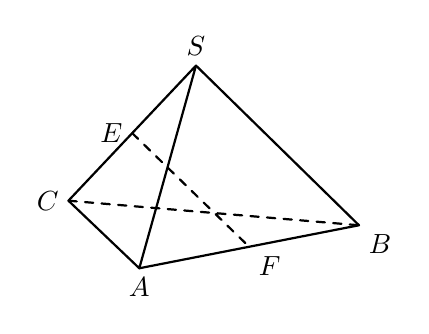
\begin{tikzpicture}[x=0.9cm,y=0.78cm,line cap=round,line join=round]
  \coordinate (S) at (0.8,3.3);
  \coordinate (A) at (0,0);
  \coordinate (B) at (3.1,0.7);
  \coordinate (C) at (-1.0,1.1);
  \coordinate (E) at (-0.1,2.2);
  \coordinate (F) at (1.55,0.35);
  \draw[thick] (S)--(A)--(C)--(S);
  \draw[thick] (S)--(B)--(A);
  \draw[thick,dashed] (C)--(B) (E)--(F);
  \node[above] at (S) {$S$};
  \node[below] at (A) {$A$};
  \node[below right] at (B) {$B$};
  \node[left] at (C) {$C$};
  \node[left] at (E) {$E$};
  \node[below right] at (F) {$F$};
\end{tikzpicture}
\end{center}
\nopagebreak[4]
（A）$90^\circ$　　（B）$60^\circ$　　（C）$45^\circ$　　（D）$30^\circ$

\Needspace{4\baselineskip}
\textbf{解析}

\Needspace{5\baselineskip}
侧棱与底面边长相等，故这是棱长为1的正四面体。取
\nopagebreak[4]
\[
A=(0,0,0),\quad B=(1,0,0),\quad C=(\tfrac12,\tfrac{\sqrt3}{2},0),\quad S=(\tfrac12,\tfrac{\sqrt3}{6},\sqrt{\tfrac23}).
\]
\Needspace{5\baselineskip}
由中点定义，$F=(\frac12,0,0)$、$E=(\frac12,\frac{\sqrt3}{3},\frac{\sqrt6}{6})$。因此
\nopagebreak[4]
\[
\overrightarrow{EF}=(0,\tfrac{\sqrt3}{3},\tfrac{\sqrt6}{6}),\qquad
\overrightarrow{AS}=(\tfrac12,\tfrac{\sqrt3}{6},\tfrac{\sqrt6}{3}).
\]
点积为 $\frac12$，且 $|EF|=1/\sqrt2$、$|AS|=1$，故两方向夹角的余弦为 $1/\sqrt2$，所成角为 $45^\circ$。

\textbf{结论：C}

\gkanswer{答案：C}

\end{answer}
\begin{answer}
\gksolhead{15}{}

\textbf{题目}：

以一个正三棱柱的顶点为顶点的四面体共有\mbox{（　　）}。

（A）$6$ 个　　（B）$12$ 个　　（C）$18$ 个　　（D）$30$ 个

\Needspace{4\baselineskip}
\textbf{解析}

从六个顶点任取四个共有 $\binom64=15$ 组。恰有三组四点共面：它们分别是三棱柱的三个矩形侧面。去掉这三组后，其余 $15-3=12$ 组各确定一个四面体。

\textbf{结论：B}

\gkanswer{答案：B}

\end{answer}
\begin{answer}
\gksolhead{16}{}

\textbf{题目}：

已知 $\sin\alpha=\dfrac35$，$\alpha\in\left(\dfrac\pi2,\pi\right)$，那么 $\sin\dfrac\alpha2=$\gkblank{}。

\Needspace{4\baselineskip}
\textbf{解析}

\Needspace{5\baselineskip}
因为 $\alpha\in(\frac\pi2,\pi)$，所以 $\cos\alpha=-\sqrt{1-\sin^2\alpha}=-\frac45$。又 $\alpha/2\in(\frac\pi4,\frac\pi2)$，半角正弦取正值：
\nopagebreak[4]
\[
\sin\frac\alpha2=\sqrt{\frac{1-\cos\alpha}{2}}=\sqrt{\frac9{10}}=\frac3{\sqrt{10}}.
\]

\textbf{结论：$\dfrac{3}{\sqrt{10}}$}

\gkanswer{答案：$\dfrac{3}{\sqrt{10}}$}

\end{answer}
\begin{answer}
\gksolhead{17}{}

\textbf{题目}：

$(x-1)-(x-1)^2+(x-1)^3-(x-1)^4+(x-1)^5$ 的展开式中，$x^2$ 的系数等于\gkblank{}。

\Needspace{4\baselineskip}
\textbf{解析}

\Needspace{5\baselineskip}
对 $k=2,3,4,5$，$(x-1)^k$ 中 $x^2$ 项系数为 $\binom{k}{2}(-1)^{k-2}$，再乘原式中的 $(-1)^{k+1}$ 后每项均为 $-\binom{k}{2}$。所以总系数为
\nopagebreak[4]
\[
-\left[\binom22+\binom32+\binom42+\binom52\right]=-(1+3+6+10)=-20.
\]

\textbf{结论：$-20$}

\gkanswer{答案：$-20$}

\end{answer}
\begin{answer}
\gksolhead{18}{}

\textbf{题目}：

\Needspace{5\baselineskip}
已知 $\{a_n\}$ 是公差不为零的等差数列，如果 $S_n$ 是 $\{a_n\}$ 的前 $n$ 项的和，那么
\nopagebreak[4]
\[
\lim_{n\to\infty}\frac{na_n}{S_n}=
\]
\gkblank{}。

\Needspace{4\baselineskip}
\textbf{解析}

\Needspace{5\baselineskip}
设等差数列首项为 $a_1$、非零公差为 $d$。则
\nopagebreak[4]
\[
a_n=a_1+(n-1)d,\qquad S_n=\frac n2\bigl(2a_1+(n-1)d\bigr).
\]
约去 $n$ 后，分子分母最高次项之比为 $d/(d/2)=2$；$d\ne0$ 保证该极限不依赖首项。

\textbf{结论：$2$}

\gkanswer{答案：$2$}

\end{answer}
\begin{answer}
\gksolhead{19}{}

\textbf{题目}：

如果实数 $x,y$ 满足等式 $(x-2)^2+y^2=3$，那么 $\dfrac yx$ 的最大值是\gkblank{}。

\Needspace{4\baselineskip}
\textbf{解析}

\Needspace{5\baselineskip}
圆心为 $(2,0)$、半径为 $\sqrt3$。令 $m=y/x$，原圆上 $x\ne0$；过原点且斜率为 $m$ 的直线为 $y=mx$。当该直线与圆相交时，圆心到直线的距离不超过半径：
\nopagebreak[4]
\[
\frac{2|m|}{\sqrt{1+m^2}}\le\sqrt3.
\]
平方得 $m^2\le3$，且 $m=\sqrt3$ 时直线与圆相切并确有交点，故最大值为 $\sqrt3$。

\textbf{结论：$\sqrt3$}

\gkanswer{答案：$\sqrt3$}

\end{answer}
\begin{answer}
\gksolhead{20}{}

\textbf{题目}：

如图，三棱柱 $ABC-A_1B_1C_1$ 中，若 $E,F$ 分别为 $AB,AC$ 的中点，平面 $EB_1C_1F$ 将三棱柱分成体积为 $V_1,V_2$ 的两部分，那么 $V_1:V_2=$\gkblank{}。
\nopagebreak[4]
\begin{center}% 原卷第20题三棱柱及平面 EB_1C_1F；不标注未出现在原图中的体积区域名。
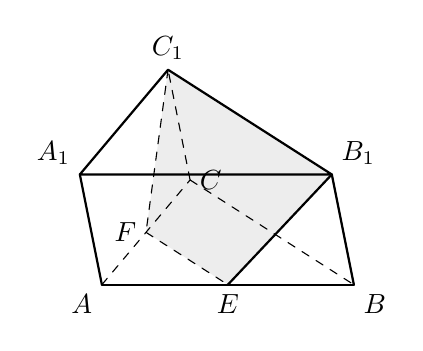
\begin{tikzpicture}[x=0.8cm,y=0.7cm,line cap=round,line join=round]
  \coordinate (A) at (0,0);
  \coordinate (B) at (4,0);
  \coordinate (C) at (1.4,1.9);
  \coordinate (Aone) at (-0.35,2.0);
  \coordinate (Bone) at (3.65,2.0);
  \coordinate (Cone) at (1.05,3.9);
  \coordinate (E) at (2,0);
  \coordinate (F) at (0.7,0.95);
  \fill[gray!14] (E)--(Bone)--(Cone)--(F)--cycle;
  \draw[thick] (A)--(B);
  \draw[thick] (Aone)--(Bone)--(Cone)--(Aone);
  \draw[thick] (A)--(Aone) (B)--(Bone);
  \draw[dashed] (A)--(C) (C)--(Cone) (C)--(B) (Cone)--(F) (F)--(E);
  \draw[thick] (E)--(Bone);
  \node[below left] at (A) {$A$};
  \node[below right] at (B) {$B$};
  \node[right] at (C) {$C$};
  \node[above left] at (Aone) {$A_1$};
  \node[above right] at (Bone) {$B_1$};
  \node[above] at (Cone) {$C_1$};
  \node[below] at (E) {$E$};
  \node[left] at (F) {$F$};
\end{tikzpicture}
\end{center}
\nopagebreak[4]
\Needspace{4\baselineskip}
\textbf{解析}

\Needspace{5\baselineskip}
令三棱柱的底面积为 $A$、高为 $H$，并以 $t\in[0,1]$ 表示从底面到顶面的高度比例。在高度 $t$ 的平行截面中，分割线端点分别从 $E,F$ 向 $B,C$ 线性移动；靠 $A$ 一侧小三角形的两条边相对 $AB,AC$ 的比例均为 $(1+t)/2$，故该侧截面积占底面积的比例为 $(1+t)^2/4$。体积积分为
\nopagebreak[4]
\[
V_A=AH\int_0^1\frac{(1+t)^2}{4}\,dt=\frac7{12}AH,
\qquad V_{\mathrm{other}}=\frac5{12}AH.
\]
因此只能确定 $A$ 侧:另一侧 $=7:5$。固定源图没有标明哪一侧记作 $V_1$，哪一侧记作 $V_2$；擅自指定会把两个合法次序之一误写为原题唯一答案。

\textbf{结论：待核（A侧:其余=7:5；V1/V2顺序未标）}

\gkanswer{答案：待核（A侧:其余=7:5；V1/V2顺序未标）}

\end{answer}
\begin{answer}
\gksolhead{21}{}

\textbf{题目}：

有四个数，其中前三个数成等差数列，后三个数成等比数列，并且第一个数与第四个数的和是 $16$，第二个数与第三个数的和是 $12$。求这四个数。

\Needspace{4\baselineskip}
\textbf{解析}

\Needspace{5\baselineskip}
设第二个数为 $m$、等差公差为 $d$，则四数为 $m-d,m,m+d,x_4$。由后面三数成等比数列，$m x_4=(m+d)^2$。第二、三数和给出 $2m+d=12$；因此 $m\ne0$，并可写 $x_4=(m+d)^2/m$。将第一、四数和代入：
\nopagebreak[4]
\[
m-d+\frac{(m+d)^2}{m}=2m+d+\frac{d^2}{m}=16.
\]
利用 $2m+d=12$ 得 $d^2=4m$。消去 $m$ 后，$d^2+2d-24=0$，所以 $(d,m)=(4,4)$ 或 $(-6,9)$。对应四数分别是 $(0,4,8,16)$、$(15,9,3,1)$。

\textbf{结论：$\{(0,4,8,16),(15,9,3,1)\}$}

\gkanswer{答案：$\{(0,4,8,16),(15,9,3,1)\}$}

\end{answer}
\begin{answer}
\gksolhead{22}{}

\textbf{题目}：

已知 $\sin\alpha+\sin\beta=\dfrac14$，$\cos\alpha+\cos\beta=\dfrac13$，求 $\tan(\alpha+\beta)$ 的值。

\Needspace{4\baselineskip}
\textbf{解析}

\Needspace{5\baselineskip}
令 $u=(\alpha+\beta)/2$、$v=(\alpha-\beta)/2$。由和差化积，
\nopagebreak[4]
\[
\sin\alpha+\sin\beta=2\sin u\cos v=\frac14,\qquad
\cos\alpha+\cos\beta=2\cos u\cos v=\frac13.
\]
\Needspace{5\baselineskip}
两式相除得 $\tan u=3/4$。于是
\nopagebreak[4]
\[
\tan(\alpha+\beta)=\tan(2u)=\frac{2(3/4)}{1-(3/4)^2}=\frac{24}{7}.
\]

\textbf{结论：$\dfrac{24}{7}$}

\gkanswer{答案：$\dfrac{24}{7}$}

\end{answer}
\begin{answer}
\gksolhead{23}{}

\textbf{题目}：

如图，在三棱锥 $S-ABC$ 中，$SA\perp$ 底面 $ABC$，$AB\perp BC$。$DE$ 垂直平分 $SC$，且分别交 $AC,SC$ 于 $D,E$。又 $SA=AB$，$SB=BC$。求以 $BD$ 为棱、以 $BDE$ 与 $BDC$ 为面的二面角的度数。
\nopagebreak[4]
\begin{center}% 原卷第23题三棱锥；虚实线及标号按固定源重绘，投影不表示长度比例。
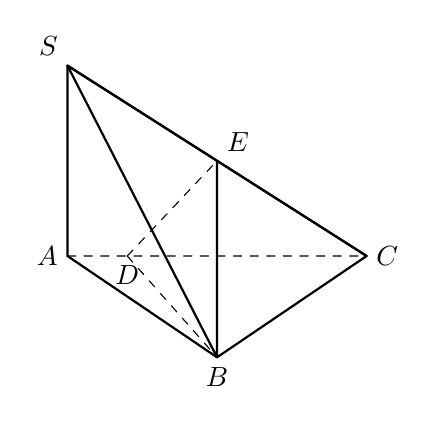
\begin{tikzpicture}[x=0.95cm,y=0.78cm,line cap=round,line join=round]
  \coordinate (A) at (-1.6,0);
  \coordinate (C) at (2.4,0);
  \coordinate (B) at (0.4,-1.65);
  \coordinate (S) at (-1.6,3.1);
  \coordinate (D) at (-0.8,0);
  \coordinate (E) at (0.4,1.55);
  \draw[thick] (A)--(S)--(C)--(B)--cycle;
  \draw[thick] (S)--(B) (S)--(E) (E)--(C) (E)--(B);
  \draw[dashed] (A)--(C) (D)--(B) (D)--(E);
  \node[above left] at (S) {$S$};
  \node[left] at (A) {$A$};
  \node[below] at (B) {$B$};
  \node[right] at (C) {$C$};
  \node[below] at (D) {$D$};
  \node[above right] at (E) {$E$};
\end{tikzpicture}
\end{center}
\nopagebreak[4]
\Needspace{4\baselineskip}
\textbf{解析}

\Needspace{5\baselineskip}
设 $AB=SA=a$。取直角底面坐标 $B=(0,0,0)$、$A=(a,0,0)$、$C=(0,\sqrt2a,0)$；由 $SB=BC=\sqrt2a$ 且 $SA\perp$底面，取 $S=(a,0,a)$。设 $D$ 在 $AC$ 上：$D=(a(1-t),\sqrt2at,0)$。因为 $E$ 是 $SC$ 中点且 $DE\perp SC$，由 $(D-E)\cdot(C-S)=0$ 得 $t=1/3$。因此
\nopagebreak[4]
\[
D=(\tfrac{2a}{3},\tfrac{\sqrt2a}{3},0),\quad
\overrightarrow{DC}=(-\tfrac{2a}{3},\tfrac{2\sqrt2a}{3},0),\quad
\overrightarrow{DE}=(-\tfrac a6,\tfrac{\sqrt2a}{6},\tfrac a2).
\]
向量 $DC$、$DE$ 都垂直于棱 $BD$，可直接作为垂直于棱的截面内两射线。其点积为 $a^2/3$，模长分别为 $2a/\sqrt3$ 和 $a/\sqrt3$，故夹角余弦为 $1/2$，二面角为 $60^\circ$。

\textbf{结论：$60^\circ$}

\gkanswer{答案：$60^\circ$}

\end{answer}
\begin{answer}
\gksolhead{24}{}

\textbf{题目}：

\Needspace{5\baselineskip}
已知 $a>0$，$a\ne1$，解不等式：
\nopagebreak[4]
\[
\log_a(4+3x-x^2)-\log_a(2x-1)>\log_a2.
\]

\Needspace{4\baselineskip}
\textbf{解析}

\Needspace{5\baselineskip}
定义域要求 $4+3x-x^2>0$ 且 $2x-1>0$，所以 $\frac12<x<4$。合并对数后比较
\nopagebreak[4]
\[
\log_a\frac{4+3x-x^2}{2x-1}>\log_a2.
\]
若 $a>1$，对数递增，等价于 $4+3x-x^2>4x-2$，即 $(x+3)(x-2)<0$；与定义域相交得 $\frac12<x<2$。若 $0<a<1$，对数递减，不等号反向，得到 $(x+3)(x-2)>0$；与定义域相交得 $2<x<4$。

\textbf{结论：$a>1:(\frac12,2);\ 0<a<1:(2,4)$}

\gkanswer{答案：若 $a>1$，$x\in(\frac12,2)$；若 $0<a<1$，$x\in(2,4)$}

\end{answer}
\begin{answer}
\gksolhead{25}{}

\textbf{题目}：

\Needspace{5\baselineskip}
设 $a\ge0$，在复数集 $\mathbb C$ 中解方程：
\nopagebreak[4]
\[
z^2+2|z|=a.
\]

\Needspace{4\baselineskip}
\textbf{解析}

设 $z=x+iy$。虚部条件为 $2xy=0$，故 $x=0$ 或 $y=0$。

若 $y=0$，令 $r=|x|$，则 $r^2+2r=a$，所以 $r=\sqrt{1+a}-1$，得到 $z=\pm(\sqrt{1+a}-1)$（当 $a=0$ 时两符号给出同一点 $z=0$）。

若 $x=0$，令 $r=|y|$，则 $-r^2+2r=a$。有实数解的条件为 $0\le a\le1$，且 $r=1\pm\sqrt{1-a}$，故另有 $z=\pm i(1\pm\sqrt{1-a})$；当 $a=0$ 时其中 $r=0$ 对应 $z=0$，不重复计数。

\textbf{结论：$z=\pm(\sqrt{1+a}-1)$；$0\le a\le1$ 时另有 $z=\pm i(1\pm\sqrt{1-a})$}

\gkanswer{答案：对任意 $a\ge0$ 有 $z=\pm(\sqrt{1+a}-1)$；若 $0\le a\le1$，另有 $z=\pm i(1\pm\sqrt{1-a})$}

\end{answer}
\begin{answer}
\gksolhead{26}{}

\textbf{题目}：

设椭圆的中心是坐标原点，长轴在 $x$ 轴上，离心率 $e=\dfrac{\sqrt3}{2}$。已知点 $P\left(0,\dfrac32\right)$ 到这个椭圆上的点的最远距离是 $\sqrt7$。求这个椭圆的方程，并求椭圆上到点 $P$ 的距离等于 $\sqrt7$ 的点的坐标。

\Needspace{4\baselineskip}
\textbf{解析}

\Needspace{5\baselineskip}
设长、短半轴分别为 $A,B$。由 $e^2=1-B^2/A^2=3/4$ 得 $B=A/2$。参数化椭圆：$x=A\cos t$、$y=B\sin t$，令 $u=\sin t\in[-1,1]$，到 $P=(0,3/2)$ 的距离平方为
\nopagebreak[4]
\[
d^2=A^2(1-u^2)+(Bu-\tfrac32)^2
=A^2+\frac94-\frac{3A^2}{4}u^2-\frac{3A}{2}u.
\]
这是关于 $u$ 的开口向下二次函数，顶点为 $u=-1/A$。若 $A\le1$，最大值在 $u=-1$，距离至多 $A/2+3/2\le2$，与给定最大距离 $\sqrt7>2$ 矛盾；故 $A>1$，顶点落在 $[-1,1]$ 内。此时最大距离平方为 $A^2+3=7$，得 $A=2,B=1$。

再与圆 $x^2+(y-\frac32)^2=7$ 联立椭圆 $x^2/4+y^2=1$，消去 $x^2$ 得 $3(y+\frac12)^2=0$，所以 $y=-\frac12$、$x=\pm\sqrt3$。

\textbf{结论：$\frac{x^2}{4}+y^2=1$；$(\pm\sqrt3,-\frac12)$}

\gkanswer{答案：椭圆方程为 $\dfrac{x^2}{4}+y^2=1$；所求点为 $(\sqrt3,-\frac12)$、$(-\sqrt3,-\frac12)$}

\end{answer}